\documentclass[11pt]{article}
%\usepackage{colacl}
\usepackage{graphicx}
\sloppy

%\usepackage{natbib}
\usepackage[nottoc]{tocbibind}
\usepackage[top=1cm,bottom=1.5cm,left=1cm,right=1cm]{geometry}
\usepackage{amsmath}
\usepackage{cases}
\usepackage{float}
\usepackage{stfloats}
\usepackage{caption}
\usepackage{subcaption}
\usepackage{fancyvrb}
\usepackage{tabularx}
\usepackage{dirtree}
\usepackage{lipsum}
\usepackage{ragged2e}
\usepackage{multicol}
\usepackage{tcolorbox}
\usepackage{hyperref}
\usepackage{setspace}
\setcounter{MaxMatrixCols}{20}
\setcounter{secnumdepth}{2}

\usepackage{listings}
\usepackage{xcolor}

\definecolor{codegreen}{rgb}{0,0.6,0}
\definecolor{codegray}{rgb}{0.5,0.5,0.5}
\definecolor{codepurple}{rgb}{0.58,0,0.82}
\definecolor{backcolour}{rgb}{0.95,0.95,0.92}

\lstdefinestyle{mystyle}{
    backgroundcolor=\color{backcolour},   
    commentstyle=\color{codegreen},
    keywordstyle=\color{magenta},
    numberstyle=\tiny\color{codegray},
    stringstyle=\color{codepurple},
    basicstyle=\ttfamily\footnotesize,
    breakatwhitespace=false,         
    breaklines=true,                 
    captionpos=b,                    
    keepspaces=true,                 
    numbersep=5pt,                  
    showspaces=false,                
    showstringspaces=false,
    showtabs=false,                  
    tabsize=2
}
 \hypersetup{
     colorlinks=true,
     linkcolor=blue,
     filecolor=blue,
     citecolor=black,      
     urlcolor=black,
     }

\lstset{style=mystyle}

\renewcommand{\familydefault}{\sfdefault}

\title{\vspace{-1cm}\bf\large COMP90086 Computer Vision - Final Project\\\LARGE Fine-grained Localisation}
\author{Tuan Khoi Nguyen (1025294) \hspace{3cm} Hoang Anh Huy Luu (1025379)\\
        %\it Word Count: 2496 (Excluding Tables, Figures and References)
        }

%\setlength{\parindent}{1em}
%\setlength{\parskip}{0.5em}
\renewcommand{\baselinestretch}{0.9}
\begin{document}
\maketitle
%\setlength{\columnsep}{100pt}
\setlength{\columnsep}{1.5cm}
\setlength{\columnseprule}{0.5pt}

%\section{Introduction}
\vspace{-0.5cm}
\renewcommand{\abstractname}{Introduction}
\begin{abstract}
\noindent In Computer Vision, image localisation is common for locating exactly where a picture is taken. This report will describe the group's systematic process of building the localisation model for 1200 images in the Getty Center in Los Angeles, USA, with the approaches containing a mixture between traditional feature extraction methods and new evaluation ideas, which resulted in some of our notable self-developed methods such as \textbf{Joint Adversarial Validation (JAV)}, \textbf{CumuLative Online Clustered K-Means (CLOCK)} and \textbf{Similar Histogram Online Clustered K-Means (SHOCK)}. These models have proven to be effective, and helped us in outperforming most competitors in \hyperlink{https://www.kaggle.com/c/comp90086-2021/overview}{The Kaggle Leaderboard} \footnote{Ranked 3rd over 212 competing teams, as of October 22nd 2021}.
\end{abstract}
%\vspace{0.2cm}

\begin{multicols}{2}
\section{Overview}
With the output requiring coordinates in the form of \texttt{(x,y)}, this task can be seen in common problem types of geolocation or geotagging. This suggests solving directions of taking in spatial information such as object presence and color distribution, or neighboring information such as the location of a similar picture.
\vspace{-0.2cm}
\subsection*{The Data}
\vspace{-0.5cm}
\begin{figure}[H]
    \centering
    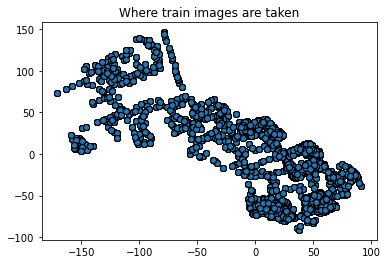
\includegraphics[width=0.35\textwidth]{Project/train_distribution.png}
    \caption{The location distribution of training dataset}
    \label{fig:train}
\end{figure}

\noindent Resulting plot from Figure \ref{fig:train} shows that the distribution for each data is diverse. While some locations have dense amount of images, some other areas have little to none images taken. This may result in conventional models not generalising well when a location has too few information known, or easily mistaken to another dense area with slight similarities. It is also noticeable that the data is only 2-dimensional, which may result in different views located within the same area due to elevation differences.

\section{Process Methods \& Learner Models}
\noindent The following section lists the learners used in this project. Given the task and data overview, the learners will focus on finding similarity criteria to match the test instances to their most similar train instance, and further test the approximation with translation algebra. It will also lists methods that aims in validating the data representation of the test set respective to train set, and getting the optimal set of hyperparameters.


\vspace{-0.4cm}
\subsection{Validation \& Hyperparameter Tuning}

\paragraph{Joint Adversarial Validation (JAV)} To ensure accurate validation, assessment criteria for data representation is vital. Adversarial validation \cite{Pan2020AdversarialVA} measures similarity in distribution between 2 datasets, by attempting to distinguish them with a binary classification model. Lower accuracy means that the datasets have similar distribution, which makes each dataset being well-represented to the other. In order to pick the a validation set that will represent the testing dataset well, the candidate validation sets will have its train set representation compared against that of test set to get the most reflecting validation accuracy. 

\vspace{-0.4cm}
\paragraph{2-Layer Grid Search} With large number of hyperparameters and limited time constraint, it is impractical to do a full grid search by going through each combination in small steps. Therefore, 2-Layer Grid Search, which selects combinations in longer steps to run the validation on, is chosen as the tuning method for this task. \\~\\
The process will be done first on a large pool of combinations with large steps, picking the best combination, then narrow the search down to smaller steps, on surrounding candidates close to that combination.

\subsection{Single Models}
Except for the baselines, these models will all aim to assess similarity to pick the most similar images. Currently, the average location of these images will be taken.
\vspace{-0.4cm}
\paragraph{Center Allocation, Random Allocation (Baseline)} The former will assign the mean of all training locations to all test instances, while the latter allocate the locations randomly within training location range. These 2 allocations methods rarely use dataset information, hence chosen as the minimum baseline for other models.
\vspace{-0.4cm}
\paragraph{Convolutional Neural Network (CNN - Benchmark)} CNN is the commonly used method for many computer vision tasks, which works by using pre-trained image datasets to extract image features. The model is chosen as the benchmark for its common use and well-known performance \cite{cnn}. A number of different CNN models will be tested, each taking the final fully connected layer as the output to ensure that useful features are kept, while maintaining reasonable memory usage. The extraction result will measure similarity using Euclidean's Distance.
\vspace{-0.4cm}
\paragraph{Scale Invariant Feature Transform (SIFT)} SIFT works by matching similar patterns from color gradients, and count the number of matches \cite{sift}. For this task, SIFT will be used with Fast Library for Approximate Nearest Neighbors (FLANN) and filtered on Lowe's Ratio Test \cite{Lowe}. The similarity criteria is the number of matching points that passed the ratio test.

\subsection{Ensemble Models}
\noindent With the single models found and chosen, we attempted to improve on these models with combinations and modifications. Using model evaluation and domain knowledge, we have developed a number of extension or combination models for the localization problem.
\vspace{-0.4cm}
\paragraph{CumuLative Online Clustered K-Means (CLOCK)} Noting that the top candidates may include outliers, a dynamic clustering method is introduced. This method allocates the instances to clusters sequentially by getting one's distance to the centroids, and create a new cluster for every instace that is too far away. When having enough clusters or instances, the biggest cluster is chosen and its centroid will be determined as the final location.
\vspace{-0.4cm}
\paragraph{CNN + SIFT (Combination)} Noting that each singular model has their own weakness (which will be discussed after the Results section), we come up with the idea of sequential filtering. After filtering out weak images with CNN similarity, the model then rank the rest by SIFT matches, and use CLOCK to get the best average.
\vspace{-0.4cm}
\paragraph{Similar Histogram Online Clustered K-Means (SHOCK)} With the domain knowledge that all images are taken from the same camera, it can be assumed that images from the same area should share the same image colors. Therefore, color is chosen as an additional similarity criteria to filter out the outliers from CNN and SIFT. The number of histogram intersections is the similarity measurement, with larger number corresponding to more color-similar image.\\~\\
It is noted that each similarity criteria has its own weakness that result in wrong prediction in small cases that can be omitted by other criteria, CLOCK clustering algorithm is expanded. Rather than choosing the biggest cluster, the model will vote between the biggest cluster, the cluster with the best SIFT matches, and the cluster with the most color matches.

\paragraph{Transform Calculation} Now with the approximated location and the surrounding image cluster calculated for each image through CLOCK, and the domain knowledge that all images are taken with the same camera, the exact location can now be calculated using SIFT matching points and epipolar geometry. Further mathematical details will be described in Appendix \ref{translation}.

\section{Setting Up}

\paragraph{Operating Environment \& Adaption} The training process will be done concurrently across 3 devices to cut down running time and memory storage. Furthermore, to adapt to similar environments that lack resources, our implementation are built with the following attributes:
\begin{itemize}
    \item Ability to run on any data partition rather than requiring the whole dataset. This way, training process can be divided across multiple devices.
    \item The process will export data segments to hard drive, and read them in again when needed, rather than storing them in memory. This way, the memory constraint is solved, and the procedure can always resume if there is a disconnection halfway. 
\end{itemize}

\paragraph{Data Engineering \& Storage} Given that the size for each picture is large, we proceed to extract the essential features in a variety of ways to give our models good head start. We were able to extract features in 2 ways: using pre-trained CNN models, or SIFT matching. The images will then have their extracted features compared against training instances, then ranked and store to \texttt{.csv} files.

\paragraph{Validation} While Kaggle public data contains 50\% of the dataset, we were not able to fully evaluate model performance due to the submission limit, hence needed another validation method to rely. Given time constraint, we can only run validation process on partial data. Therefore, JAV is used as the assessing criteria, so that the chosen partition's experimentation results can be as reflective as possible for test set. The best data subset of 1/12 Hold-out (600 instances) will then be preserved for validation.

\paragraph{Hyperparameters} Setting hyperparameters is done for CLOCK and SIFT, which have short running duration, has many parameters and is the base for most models. To save up the tuning process, a portion of parameters are either set to default, or chosen based on domain knowledge, namely as follows:
\begin{itemize}
    \item SIFT with FLANN matching: The parameters are based on the recommendation of Lowe's Ratio Test \cite{Lowe}: 2 Nearest Neighbors and Ratio bound of 0.7.
    \item Epipolar transforming: The minimum number of SIFT matches should be 8, to satisfy the 8-point algorithm condition \cite{8pt}.
\end{itemize}
\noindent Running 2-Layer Grid Search on the rest of parameters showing that thresholding CNN feature distance within 5 units, ensuring cluster radius less than 3, and limit of up to 3 clusters brings the most optimal solution.

\vspace{-0.3cm}
\paragraph{Model Execution} After setting up and choose suitable tuning parameters, each model will be run sequentially, with top-performing ones of each stage have their result submitted to Kaggle to estimate generalisation. Feature extraction models will be executed first to get both similarity-based predictions and information to pass on the ensembles that will be run next. After the best areas are presumably found from the ensembles, epipolar geometry is then used to attempt on estimating more precise position.

\vspace{-0.4cm}
\section{Result, Experiments \& Discussion}
%\vspace{-0cm}

\subsection{Baselines \& CNN Feature Extraction}
\noindent For all CNN models, all models will have the average location of top 3 best matching image as the final location.

\begin{table}[H]
\centering
\caption{Result of baseline and CNN models}
\vspace{-0.4cm}
\begin{tabular}{|l|l|}
\hline
\textbf{Model} & \textbf{MAE} \\ \hline
Random Allocation (Baseline) & 58.65 \\ \hline
Centre Allocation (Baseline) & 43.99 \\ \hline
VGG19 & 29.24 \\ \hline
ResNet50 &  9.82/\textbf{9.11}\\ \hline
ResNet101 & 9.74/\textbf{8.87} \\ \hline
ResNet152 &  9.90 \\ \hline
\end{tabular}
\parbox{0.45\textwidth}{\centering\small 0: 1/12 Hold-out Validation \;\; \textbf{0}: Kaggle Submission}
\end{table}

\noindent The result shows that the CNN models outperformed the baselines well as expected. Out of 4 candidates, ResNet101 were found to be the best performer, and therefore was chosen for 1st Kaggle submission and processing in further models.\\~\\
However, these CNN models have downfalls. Given that they base their similarity on features presence, which are likely present across multiples areas, the matching results can be mixed in with far away images that may cause wrong estimation.

\begin{figure}[H]
    \centering
    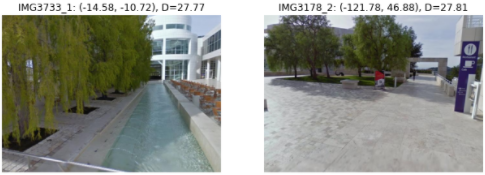
\includegraphics[width=0.45\textwidth]{Project/CNN_error.PNG}
    \caption{Faulty CNN case example}
    \label{fig:cnn}
\end{figure}

\noindent Figure \ref{fig:cnn} shows an example of the problem, where 2 pictures from different locations are considered to be similar, as they both have trees and cement ground in the scene. This proves that a more precise matching intervention such as SIFT is needed.

\subsection{SIFT}

\begin{minipage}{0.19\textwidth}
\noindent The running process shows that SIFT will not work for all instances, hence cannot produce complete output. This is because for images with no edges, SIFT will not be able to find any matching points to compare.
\end{minipage}\hfill
\begin{minipage}{0.24\textwidth}
\begin{figure}[H]
    \centering
    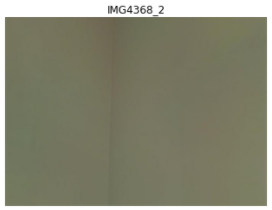
\includegraphics[width=0.85\textwidth]{Project/sift_faulty.PNG}
    \caption{An image with no SIFT matching points}
    \label{fig:sift_case}
\end{figure}
\end{minipage}\\%~\\

\noindent Error analysis also shows another problem. With some images containing noises, SIFT may mistake these noises as edge features and match them to the test instances, as shown in Figure \ref{fig:sift}. Therefore, SIFT cannot run on it's own, and will need imputation or combination with a different model to eliminate these noisy images first.

\begin{figure}[H]
    \centering
    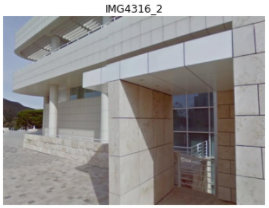
\includegraphics[width=0.2\textwidth]{Project/SIFT_error1.PNG}
\end{figure}
\vspace{-1cm}
\begin{figure}[H]
    \centering
    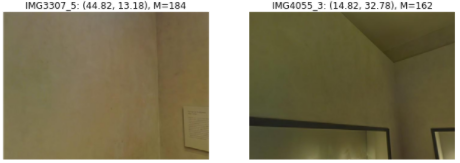
\includegraphics[width=0.45\textwidth]{Project/SIFT_error2.PNG}
    \caption{Case example of an image found to be best matched with different noisy wall images}
    \label{fig:sift}
\end{figure}

\subsection{Ensembles}

\begin{table}[H]
\centering
\caption{Result table of ensemble models}
\vspace{-0.4cm}
\begin{tabular}{|l|l|l|}
\hline
\textbf{Model} & \textbf{Estimation Method} & \textbf{MAE} \\ \hline
CNN & Top 3 Average & 9.74/\textbf{8.87} \\ \hline
CNN & CLOCK & 7.96/\textbf{7.67} \\ \hline
CNN + SIFT & Top 1 Average & 4.59 \\ \hline
CNN + SIFT & CLOCK & 4.22 \\ \hline
CNN + SIFT & SHOCK & 3.86/\textbf{3.90} \\ \hline
CNN + SIFT & SHOCK + Epipolar & 4.12/\textbf{4.06} \\ \hline
\end{tabular}
\parbox{0.45\textwidth}{\centering\small Chosen CNN Model: ResNet101}
\parbox{0.45\textwidth}{\centering\small 0: 1/12 Hold-out Validation \;\; \textbf{0}: Kaggle Submission}
\end{table}

\paragraph{CLOCK \& Combination Model} As expected, CLOCK worked well in eliminating outlier estimations, and improved the outcome for both CNN \& combination model. The combination model also proven to perform better than single CNN model, after crossing out irrelevant locations with SIFT matches. However, relying fully on identical features also have downfalls in some cases, especially when different viewing angles can return different textures or panorama stitches, resulting in detail loss.

\begin{figure}[H]
    \centering
    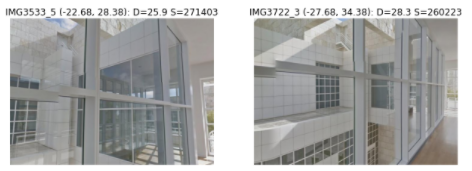
\includegraphics[width=0.45\textwidth]{Project/diffviews.PNG}
    \caption{Different orientations returning different details}
    \label{fig:diff}
\end{figure}

\noindent Figure \ref{fig:diff} shows an example of the case. Not only the window frame details are not in shape due to the panorama stitch, when looking at closer view on the left, new grid texture started to appear on side window due to glass reflection, making the picture being less recognizable than the other picture. This is when the color similarity comes in handy, where it can detect the similar color tones through histogram intersections, given the domain knowledge that the tone within an area should be identical.

\paragraph{SHOCK} After taking color tone into consideration, the error is slightly reduced. This model is now presumed to produce the most precise approximated location for the test set, with mean error of 3.9 on Kaggle public dataset. However, some problems are still remaining.
\begin{figure}[H]
    \centering
    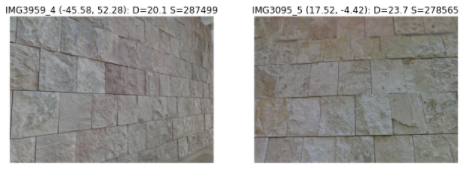
\includegraphics[width=0.45\textwidth]{Project/texture.PNG}
    \caption{Identical textures in different locations}
    \label{fig:texture}
\end{figure}
\noindent Error analysis shows that like Figure \ref{fig:texture}, there are different locations sharing the same textures, which is common in wall images. Even human perception can hardly distinguish between these textures. Potential solutions to this problem may include high-level edge detection to find smaller visible details, or even using lighting geometry and image brightness to predict the taken location. However, with the time and resource constraint, these methods becomes infeasible, and can only be considered in the future where the conditions are more ready.

\begin{figure}[H]
    \centering
    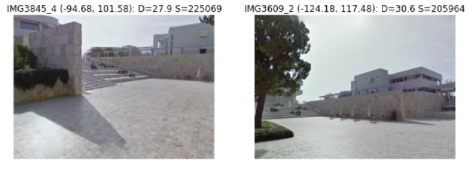
\includegraphics[width=0.45\textwidth]{Project/farview.PNG}
    \caption{Identical outdoor views that are far away}
    \label{fig:far}
\end{figure}
\noindent Another problem that is common in outdoor view, shown in Figure \ref{fig:far} is that while 2 images can share the same details, they might be actually far away, given that the camera center can point to infinity. Therefore, epipolar geometry is believed to solve this problem, by estimating the translation vector between images.

\paragraph{Epipolar Geometry} Contrary to expectation, the result with epipolar geometry not only showed no improvement, but also slightly decrease the performance. This shows that the outdoor view problem is not actually common in this dataset. Furthermore, with the current best mean error of 3.9, the algorithm is likely to have uncertainty that exceeded this value, making the estimation useless. Regardless of this, the algorithm will still become useful when more outdoor images are put into the dataset.

\subsection{Potential Improvements}
\noindent While our current model performed quite well on the dataset, there are still potentals remaining to improve the task, which were not able to be implemented due to the limit on data, time and resources. These includes panorama stitching images at the same area to make features more visible as a whole, or make a dynamic algorithm that changes parameters based on whether image is identidied as outdoors or indoors. Validation could also be done more completely with cross-validation, and rerun multiple times to give a more stable estimation.

\section{Conclusion \& Directions}
\noindent Overall, through experimentation and error analysis, we came up with the ensemble model SHOCK, which consist of similarity detection using CNN features, SIFT matches and color histograms, and processed with CLOCK clustering method. This model has proven to perform effictively for the dataset, taking us to the top percentile of the Kaggle leaderboard. There will be even more space for development when more time and data are available.\\~\\
With the locations now detected for each image, possible developments may include using Simultaneous Localization and Mapping (SLAM) to construct 3D views for the Getty Center, or even use the newly predicted instances to fill in the panorama stitches, making the Google Maps Street View better for user experience.


\newpage
\bibliographystyle{unsrt}
\bibliography{proj}

\appendix
\section{Translation Method}\label{translation}

\subsection{Intrinsic Camera Matrix}
\noindent With Field of View $(FOV_x,FOV_y)$ and size of image in pixels $(w,h)$ given, the intrinsic camera matrix can be found as follows, assuming pinhole camera model:
\[K = 
\begin{bmatrix}
\frac{w}{2tan(0.5 \times FOV_x)} & 0 & \frac{w}{2}\\
0 & \frac{h}{2tan(0.5 \times FOV_y)} & \frac{h}{2}\\
0 & 0 & 1 
\end{bmatrix}
\]

\subsection{Translation Algebra}
\begin{figure}[H]
    \centering
    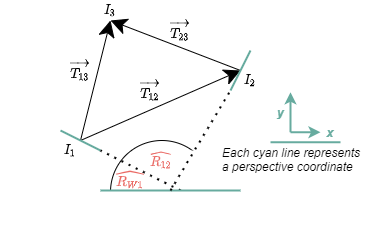
\includegraphics[width = 0.45\textwidth]{Project/cvproj.drawio.png}
    \vspace{-1.5cm}\caption{Arrangement diagram of epipolar geometry}
    \label{fig:translation}
\end{figure}
\noindent This method requires at least 2 images $I_1,I_2$ with known coordinates to get the 3rd coordinate for image $I_3$, with each image having at least 8 point matches to perform the 8-Point Algorithm. \\~\\
\columnbreak
Assuming that the elevation is always the same. This way, any 2D real-world translation of $(x,y)$ can be represented in 3D space as $T = \begin{bmatrix}
x\\0\\y
\end{bmatrix}$. For each pair of coordinates, the process can be done as follows:
\begin{itemize}
    \item With $K$ achieved, find the essential matrix $E_{12}$ between $I_1,I_2$
    \item Decompose $E_{12}$, get rotation matrix $R_{12}$ and translation matrix $T_{12}$ to get from $I_2$ to $I_1$, in $I_1$ world coordinates.
    \item Get the angle of the translation vector $T_{12}$, in both $I_1$ coordinates and real-world coordinates $W$, using $arctan$ formula.
    \item Get the angle difference $\theta$ between 2 world coordinates, and get its rotation vector $R_{W1}$.
    \item Unit translation vectors to $I_3$ can now be calculated in real world coordinates: 
    \begin{align*}
        T_{13} &= R_{W1}T_{13 (I1)}\\
        T_{23} &= R_{W1}R_{12}T_{23 (I1)}
    \end{align*}
    \item Form vector equation: $x_1T_{13} + x_2T_{23} = T_{12}$. 
    \item Solve $\begin{bmatrix}
    \vert & \vert & \vert \\
    T_{13} & 0 & T_{23}\\
    \vert & \vert & \vert 
    \end{bmatrix}
    \begin{bmatrix}
    x_1\\0\\
    x_2
    \end{bmatrix} = T_{12}$
    \item Get image coordinate $I_3 = I_1 - x_1T_{13}$
\end{itemize}

\noindent For more than 2 known images, do this process for each unique pair, and put the results to CLOCK clustering to cancel out erroneous predictions.
%\vspace{20cm}

\end{multicols}
\end{document}
